\documentclass[]{scrartcl}
\usepackage{Preamble}

\setcounter{section}{2}
\newcommand{\exercise}{Exercise \thesection}
\newcommand{\duedate}{2020-11-23, 23:59}

\begin{document}
\section*{\exercise}

\subsection{MPI Ring Communication}
The program in \autoref{lst:ring-cpp} was used for measureing the delay between message send and receive. The slurm-batch script in \autoref{lst:ring-sbatch} was used to iterate over a different number of processes and messages.

\begin{listing}[H]
    \inputminted[firstline=8, lastline=8]{cpp}{src/ring.cpp}
    \inputminted[firstline=20, lastline=21]{cpp}{src/ring.cpp}
    \inputminted[firstline=25, lastline=34]{cpp}{src/ring.cpp}
    \inputminted[firstline=44, lastline=47]{cpp}{src/ring.cpp}
    \caption{C++ MPI Implementation for SIMD Ring Communication}%
    \label{lst:ring-cpp}
\end{listing}


\begin{listing}[H]
    \inputminted[]{bash}{slurm_ring.sh}
    \caption{SBATCH file for job tests}%
    \label{lst:ring-sbatch}
\end{listing}

These iterations rsulted in the observed per message delays as visulized in \autoref{fig:ring-msgdelay}.

\begin{figure}[ht]
    \centering
    \includegraphics[width=\linewidth]{img/ring.pdf}
    \caption{img/Ring}%
    \label{fig:ring-msgdelay}
\end{figure}

The optimal mapping with 12 processes looks ideally like in \autoref{fig:ring-opt}.

\begin{figure}[H]
    \centering
    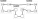
\includegraphics[width=.5\columnwidth]{img/ring-opt.pdf}
    \caption{}%
    \label{fig:ring-opt}
\end{figure}

Here each node has 4 processes (one per physical CPU core) running simultaneously, requiring three nodes.
When communicating there are two different connections:
\begin{itemize}
    \item in-node
    \item and node-to-node
\end{itemize}

While the in-node connections require a relatively small latency for message passing ($\approx \SI{1}{ms}$), the messages passed between nodes require longer to send.

To optimize the general message delay the number of node-to-node connections have to be minimized, which is three in this case.
Therefore only three in 12 messages passed per cycle require longer transmission times.

Assuming these times are constant, then we can assume that the following equeation can approximate the Messagedelay between nodes

\begin{align}
t_\text{in-node} &\approx \SI{1}{ms}\\
t_\text{avg, 2 n2n conn} &\approx \SI{36}{ms}\\
                         &=\frac 14 t_\text{n2n} + \frac 34 t_\text{in-node}\\
\Rightarrow t_\text{n2n} &\approx \SI{141}{ms}
\end{align}

$\Rightarrow$ This calculation shows that node-to-node communication is two magnitudes slower then inter-node communication.

\end{document}
